\articlehead{Shy Bladder: Why Furries Get It and How to Cure It}{JM}{2013}

Here's a scene familiar to most furries (or at least the 80\% of us that are male): visit the toilets at a public gathering and you'll see furries queueing to use a stall. Furries prefer to avoid the urinal.

[This is a pause in my article to allow the reader to creatively speculate why furries might want a stall. Come back once you're done giggling.]

This doesn't normally happen. Out in the non-furry world, there might be one or two people who prefer to use a stall, but most people are happy enough to use a urinal.

Why the difference? Because loads of furries suffer from shy bladder, otherwise known as paruresis, a condition where they will be unable to pee when someone is nearby. And as it turns out, it's an easy problem to solve.

Here's the short answer: when you're at the urinal, think about sex.

Here's why it works:

Humans are social animals. In a social group of humans, there is a hierarchy among the males. You might consider high school as an example.

The hierarchy is based on a few things, but in general the biggest, strongest, most aggressive men are the ones at the top of the social tree. Those that act gracefully and helpfully become respected leaders; those that abuse their position become bullies. In either case, those lower down will tend to defer to those higher up.

We also tend to defer to strangers: outsiders, by default, are intimidating. This is a normal social response, and a response not restricted to humans. For example male dogs will act wary around other, unfamiliar, male dogs.

We all find new people to be intimidating. You might notice that, when you meet someone new, it's difficult to make eye contact. If you are introduced by a mutual friend, you might find yourself making much more eye contact with your friend than with your new acquaintance. And when approaching a complete stranger one-on-one, it's especially difficult, because you don't have anywhere else to look.

This is worse if the stranger is taller, stronger, or otherwise deports himself in a manner that could be interpreted as being high in the social hierarchy. It's worse again if the stranger is of a different race, and worse again if his race is unfamiliar.

The act of urination is an unconscious expression of social status. There is a wealth of data collection and psychological experimentation (ref) related to urination and paruresis that demonstrates this.

You might have noticed this your own behaviour. It's easy to urinate when standing next to someone familiar that you socially dominate, perhaps a young nephew. And it's difficult if your urinal-mate is a tall, large stranger of a different race. Like, say, All Black legend Jonah Lomu.

\begin{figure}
  \begin{center}
    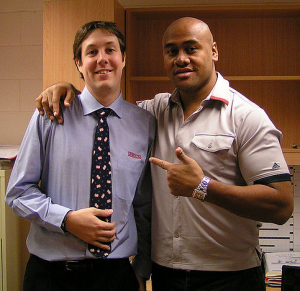
\includegraphics{content/assets/shy-bladder--1}
  \end{center}
  \caption{If Jonah follows him everywhere, the guy on the left isn't going to be able to pee for weeks. (source: Wikimedia Commons)}
\end{figure}

\begin{figure}
  \begin{center}
    
\includegraphics{content/assets/shy-bladder--2}
  \end{center}
  \caption{The guy on the left is peeing right now, but for different Jonah-Lomu-related reasons. (source: RFU hall of fame)}
\end{figure}

The solution to shy bladder is to think in a way that makes you feel like you're at the top of the social hierarchy. You can take advantage of the most basic animal instinct of all: sexual behaviour. By simply thinking about sex when you're at the urinal, you're imagining the fruits of being socially dominant. It doesn't matter if you're gay or straight, if you're thinking of a real sex act or just remembering some pornography: it's all the same to our animal brain. Just think back and recall some sort of sexual memory.

(And for the kinksters out there, or even just those who have curiously browsed /ah, it helps if you think of an unusual sex act. The weirder the better.)

It's a simple technique, and one that will come easily to most furries. We're pragmatic about sex as a general rule, and we're also familiar with thinking of ourselves as an animal.

Humans believe that they are logical beings. It's a feature of the way our brain works, and it's probably an important part of what makes us strive, as a species, to improve our lives through the getting of wisdom. But it's a false belief.

The furry identity explores this dichotomy: the conflict between our human belief in rationality and the reality of our instinct-driven animal nature. By creating an animal-person avatar, we disconnect from reality enough to explore the idea of ourselves as ideal beings.

Our furry selves tend to be extreme. We imagine ourselves engaging in idealized sexual behaviour (whatever that might be for each person), and we tend to ignore the imperfections and challenges of reality. We imagine ourselves in a physically ideal form. We imagine ourselves as successful, powerful, valuable, influential. Sometimes these idealizations are subtle; sometimes they are extreme and over-the-top.

The furry identity is a kind of roleplay, where we explore a better version of ourselves. When we spend time in the headspace of our furry identity, we're learning about our real (human, animal) desires and motivations. I have observed that younger furries tend to explore more extreme fursonas, which moderates over time into an identity more closely related to our in-real-life self.

A furry that starts with a 50-ft tall dragon fursona who rules the world and crushes all in his wake, might find himself stymied by logistical problems when emotionally connecting with people exploring less extreme furry identities. Our young furry could start spending time with a group of other 50-ft dragons, but more likely he'll moderate his fursona, perhaps to a 20-ft dragon who crushes and destroys only occasionally, when the mood takes him.

Like someone with shy bladder, or our dragon, the path to improvement often stems from an understanding of our animalistic drives. We can take advantage of our animal brain to put ourselves at ease at the urinal; we can also learn about our emotional needs by exploring an idealized version of ourselves.

In both cases, it helps to think in a way that seems irrational. Furry helps us think of ourselves as something other than a purely logical being.

There's an added bonus to this roleplay too: our idealized self -- our furry self -- provides us with an unconscious goal. The act of imagining the goal helps us see how me might achieve it.

For example: furry gymbunnies. A furry may start roleplaying a big, strong creature, and learn that such a body shape helps him feel good about himself. This might be through pride (an internal thought), or it might be through the reaction he gets from others (external influences). Our gymbunny would then think about how he can change his real-life body to match his idealized body. The furry world gives him a goal, something to work towards.

As an aside, the positive influence of goal-setting is why people think that The Secret works. \textit{The Secret}, a fleet of self-help books and films and so forth, promises that -- and this premise is so dumb that it hurts me to write -- the universe will gift you anything you desire if you simply think about whatever it is that you want.

\textit{The Secret} is, of course, world-class nonsense. But there is one positive benefit: it helps people identify a goal and use their imagination. And maybe the Secreteers, like our 50-ft dragon, will moderate their goal into something more realistic. Or maybe the Secreteers, like our gymbunny, will see the benefits of their goal and so be motivated to work towards it. (But regardless of their goal, and whatever the outcome, the Secreteers will forever be morons.)

The furry way is, at least, honest and fun and worthwhile in its own right. I don't think that imaginary furry goal-setting will translate into a successful self-help empire, Find Your Furry Fortune perhaps. But if it does, remember this: I thought of it first. Now I'm off to meditate on the idea of a nosebag full of golden oats.
